\section{Evaluation}
\label{sec:eval}
% 
\begin{figure*}[t!]
  \begin{center}
    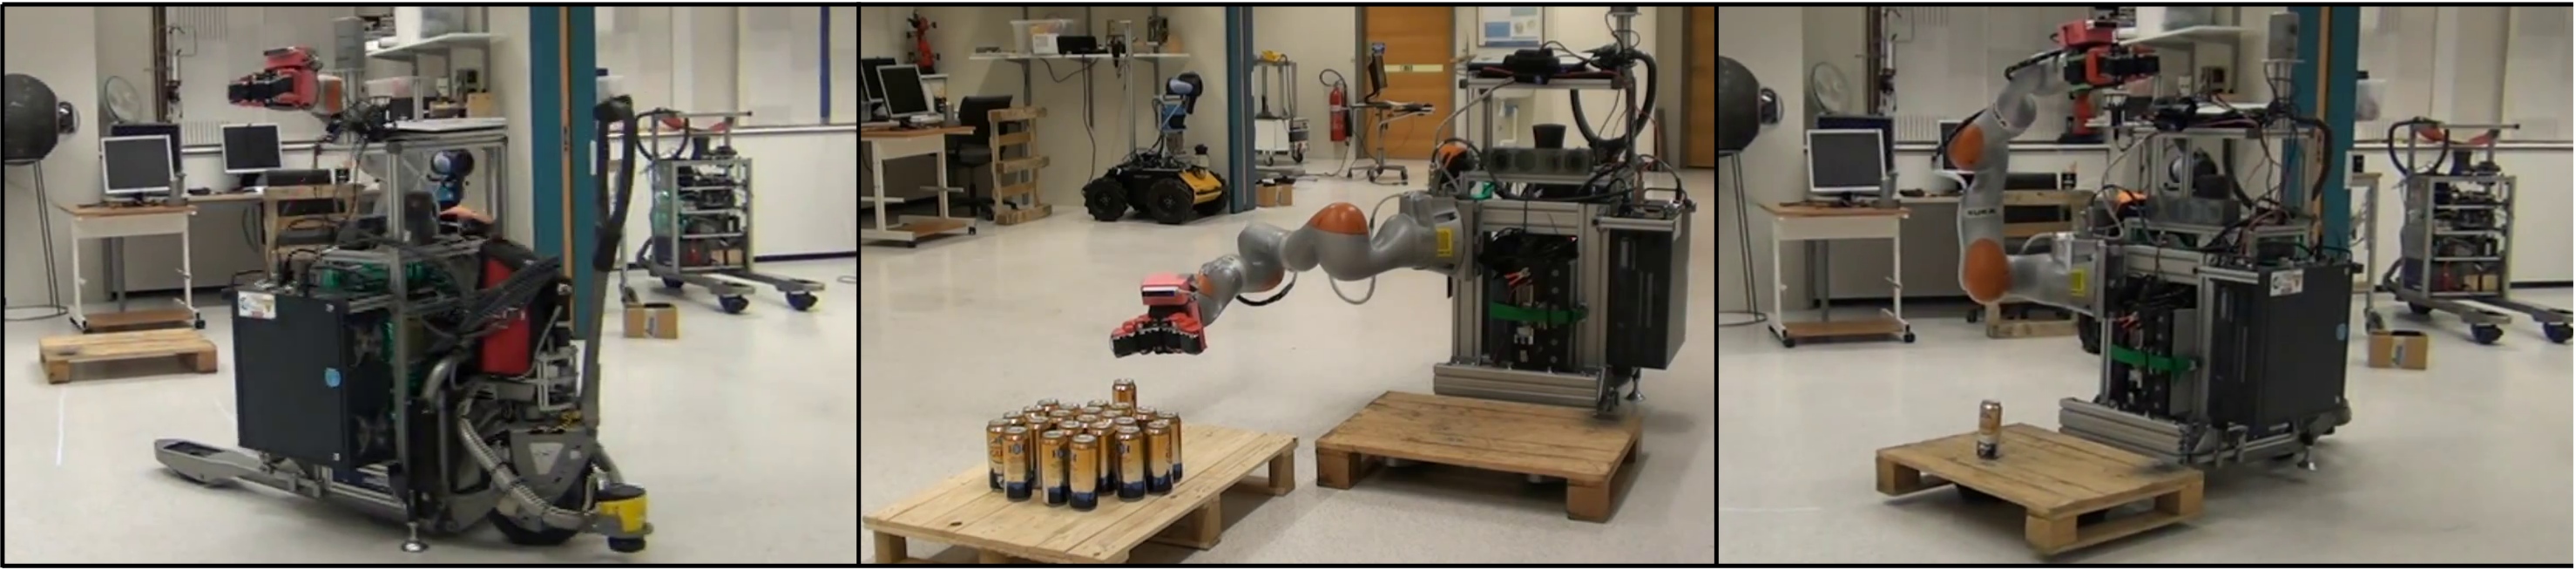
\includegraphics[width =1\linewidth]{figs/evaluation}
    % \vspace{-0.25cm}
    \caption{\textit{Evaluation setup:} (Left) the robot picks up an empty pallet in a designated
      zone; (Middle) the robot navigates to a loading zone where a can is detected and picked up;
      (Right) the loaded pallet is transported to a drop-off location.}
    \label{fig:evaluation}
    \vspace{-0.5cm}
  \end{center}
\end{figure*}
% 
For an early evaluation of the system, we set up a simplified commissioning scenario as depicted in
Fig.~\ref{fig:evaluation}. To this end, the previously described software components were
implemented in the Robot Operating System (ROS)~\cite{Quig09} framework. For manipulator motion
control (see Section~\ref{subsec:manip_motion}) we use the task function formulations
in~\cite{Kano09} for joint limit avoidance, obstacle avoidance and to formulate the inequality
constraints illustrated in Fig.~\ref{fig:truncated_grasp_interval} in order for the manipulator to
reach the grasp interval. An off-the-shelf solver~\cite{Guro15} is used to carry out the
optimizations for the motion control according to~\eqref{eq:HiQP}. The run time for the whole
procedure is approximately 4 minutes of which 2 minutes are spent on object detection and grasping
(see the attached video submission).


